\documentclass[12pt, spanish]{article}
\usepackage[spanish]{babel}
\selectlanguage{spanish}
\usepackage{natbib}
\usepackage{url}
\usepackage[utf8x]{inputenc}
\usepackage{graphicx}
\graphicspath{{images/}}
\usepackage{array}
\usepackage{float}
\usepackage{siunitx}
\usepackage[table,xcdraw,dvipsnames]{xcolor}
\usepackage{longtable}
\usepackage{parskip}
\usepackage{fancyhdr}
\usepackage{vmargin}
\usepackage{listings}
\usepackage{adjustbox}
\usepackage{subfig}
\usepackage{minted}
\usepackage[shortlabels]{enumitem}
\setlist[enumerate]{
labelsep=8pt,
labelindent=0.3\parindent,
itemindent=0pt,
leftmargin=*,
before=\setlength{\listparindent}{-\leftmargin},
}

\def\code#1{\texttt{#1}}
\usepackage[default]{sourcesanspro}
\usepackage{tcolorbox}
\usepackage{etoolbox}
\BeforeBeginEnvironment{minted}{\begin{tcolorbox}}%
\AfterEndEnvironment{minted}{\end{tcolorbox}}%

\setmarginsrb{2 cm}{1 cm}{2 cm}{2 cm}{1 cm}{1.5 cm}{1 cm}{1.5 cm}

\title{Práctica 3: Búsqueda con Adversario \\
El Parchis \hspace{0.05cm} }
\date{}
\author{
Yeray López Ramírez \\
}

\renewcommand*\contentsname{hola}

\makeatletter
\let\thetitle\@title
\let\theauthor\@author
\let\thedate\@date
\makeatother

\pagestyle{fancy}
\fancyhf{}
\rhead{}
\chead{\thedate}
\lhead{\thetitle}
\cfoot{\thepage}

\begin{document}
%%%%%%%%%%%%%%%%%%%%%%%%%%%%%%%%%%%%%%%%%%%%%%%%%%%%%%%%%%%%%%%%%%%%%%%%%%%%%%%%%%%%%%%%%
\begin{titlepage}
  \centering
  \vspace*{0.5 cm}
  
\includegraphics[scale = 0.50]{ugr.png}\\[1.0 cm]
  %\textsc{\LARGE Universidad de Granada}\\[2.0 cm]   
  \textsc{\huge Grado en Ingeniería Informática}\\[0.5 cm]
  \rule{\linewidth}{0.2 mm} \\[0.4 cm]
  { \huge \bfseries \thetitle}\\
  \rule{\linewidth}{0.2 mm} \\[1.5 cm]
  
  \begin{minipage}{0.4\textwidth}
    \begin{flushleft} \large
        \emph{Autor:}\\

        \theauthor
        \end{flushleft}
        \end{minipage}~
        \begin{minipage}{0.4\textwidth}
        \begin{flushright} \large
        \emph{Curso:2ºC \\
        Asignatura: Inteligencia Artificial \\
        Fecha: 5 de Junio de 2022
        }
    \end{flushright}
\end{minipage}\\[1 cm]


\vfill
  
\end{titlepage}

\newpage

%%%%%%%%%%%%%%%%%%%%%%%%%%%%%%%%%%%%%%%%%%%%%%%%%%%%%%%%%%%%%%%%%%%%%%%%%%%%%%%%%%%%%%%%%


\tableofcontents
\pagebreak

%%%%%%%%%%%%%%%%%%%%%%%%%%%%%%%%%%%%%%%%%%%%%%%%%%%%%%%%%%%%%%%%%%%%%%%%%%%%%%%%%%%%%%%%%

\section{Introducción}
El objetivo de esta práctica es programar en C++ un jugador de parchís dotado de una
cierta inteligencia artificial. Existen varias modalidades a la hora de jugar al parchís,
en nuestro caso es una modificación de un parchís con 4 colores y dos jugadores, de
manera que cada jugador controla una pareja de colores: amarillo/rojo para el jugador 1 y azul/verde para el jugador 2.

Se trata de un problema de búsqueda con un adversario. Dado que el parchís de base es un juego
NO determinista, no existen reglas exactas que nos lleven de forma segura a un resultado
óptimo. De hecho, en los jugadores humanos podemos observar que cada uno aplica unas determinadas reglas en función de su estilo de juego. Las reglas elegidas son lo que llamamos Heurísticas.

Nuestro objetivo en esta practica es diseñar un algoritmo de decisión: Minimax o Poda Alfa-Beta que generarán nuestro arbol de decisión del juego. También tenemos que crear una heuristica efectiva que sea capaz de vencer a tres agentes (Ninjas) creados por los propios profesores del departamento.

\section{Desarrollo}

\subsection{Estrategia MiniMax}
La estrategia mínimax consiste en elegir el mejor movimiento para el jugador (MAX) suponiendo que el adversario (MIN) escogerá el mejor para sí mismo.

El algoritmo general consta de los siguientes pasos:

\begin{enumerate}
 \item Generar el arbol de juego, alternando los movimientos de MAX y MIN, asignando el valor apropiado.

 \item Calcular la función de utilidad de cada nodo final, recorriendo el arbol recursivamente hasta volver al nodo inicial.

 \item Elegir como jugada final aquel movimiento que mayor puntuación otorge según la función de utilidad.
\end{enumerate}

La implementación del mismo para nuestro problema sería:
\begin{enumerate}
 \item Generamos el arbol de juego a través de la función generateNextMove(), alternando entre MAX y MIN con un bool MAX que se calcula con la función actual.getCurrentPlayerId(). Si es igual a jugador, significa que nos toca a nosotros en esa iteración y sino le toca al oponente.

 \item Calculamos la puntuación en los nodos terminales a través de la heurística. Un nodo terminal es una profundidad de iteración igual a la profundidad\_max que en nuestro caso es 4 o la partida en el estado actual ha acabado que se calcula con la función estado.gameOver();

 \item Se elige como jugada final los valores de id\_piece y dice que más puntuación otorge según la heurística.
\end{enumerate}

Mi implementación del mismo en código C++:

\begin{centering}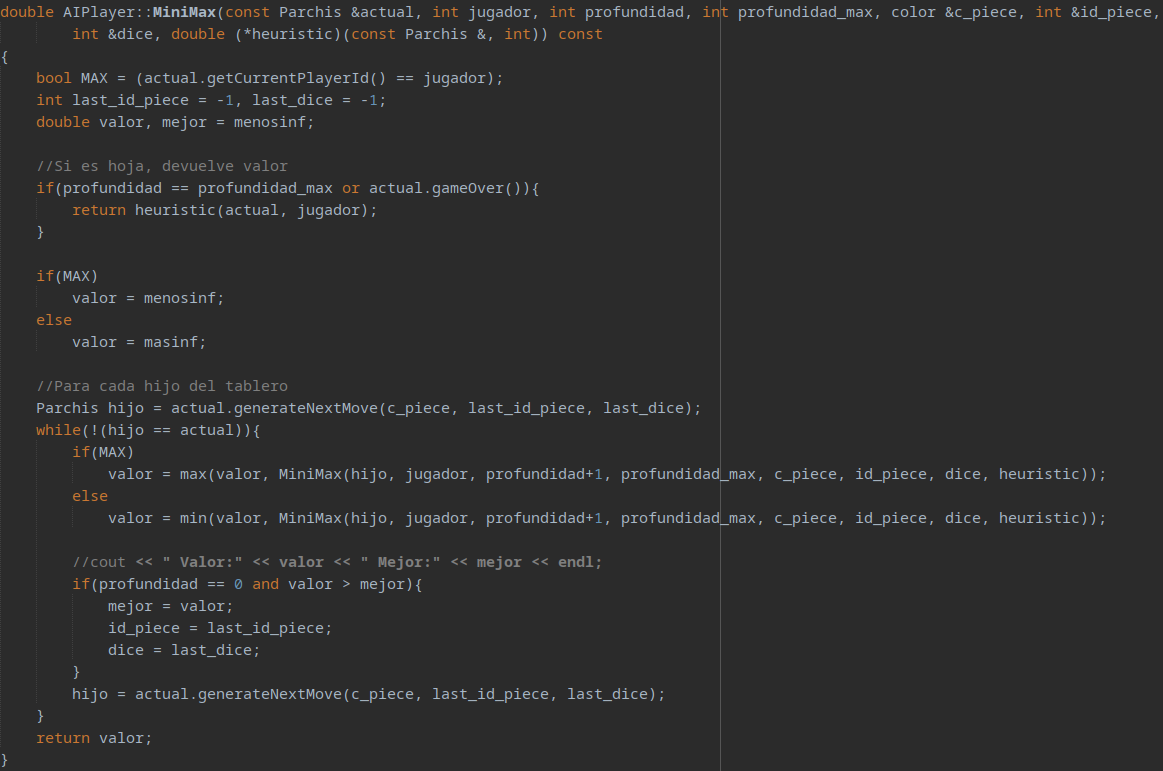
\includegraphics[scale = 0.55]{minimax.png}\\[1.0 cm]\end{centering}

\subsection{Estrategia Poda Alfa-Beta}
Sobre los árboles de juego se puede aplicar un tipo propio de poda, conocida como la Poda
alfa-beta. Es una modificación del algoritmo MiniMax donde se establecen umbrales en los nodos para descartar aquellos nodos que no los cumplan. Al adaptar la forma general para nuestro caso concreto, nos quedan los pasos:

\begin{enumerate}
 \item Si es un nodo terminal, devuelve el valor de la heurística. Para el algoritmo alfa-beta, la profundidad máxima del nodo terminal es 6 o menor si es gameOver(). En otro caso, generar el primer hijo. Si el hijo es un nodo MAX, ir al paso 2. Si es un nodo MIN ir al paso 5.
 \item Hacer alfa = max(alfa, Poda\_AlfaBeta(hijo, jugador, profundidad, profundidad\_max, ...))
 \item if(alfa >= beta) return beta; else \{continuar\}.
 \item if(hijo==actual) return alfa; else \{hijo = generatextMove()\}.
 \item Hacer beta = min(beta, Poda\_AlfaBeta(hijo, jugador, profundidad, profundidad\_max, ...))
 \item if(beta <= alfa) return alfa; else \{continuar\}.
 \item if(hijo==actual) return beta; else \{hijo = generatextMove()\}.
\end{enumerate}

La implementación del mismo en C++:

\begin{centering}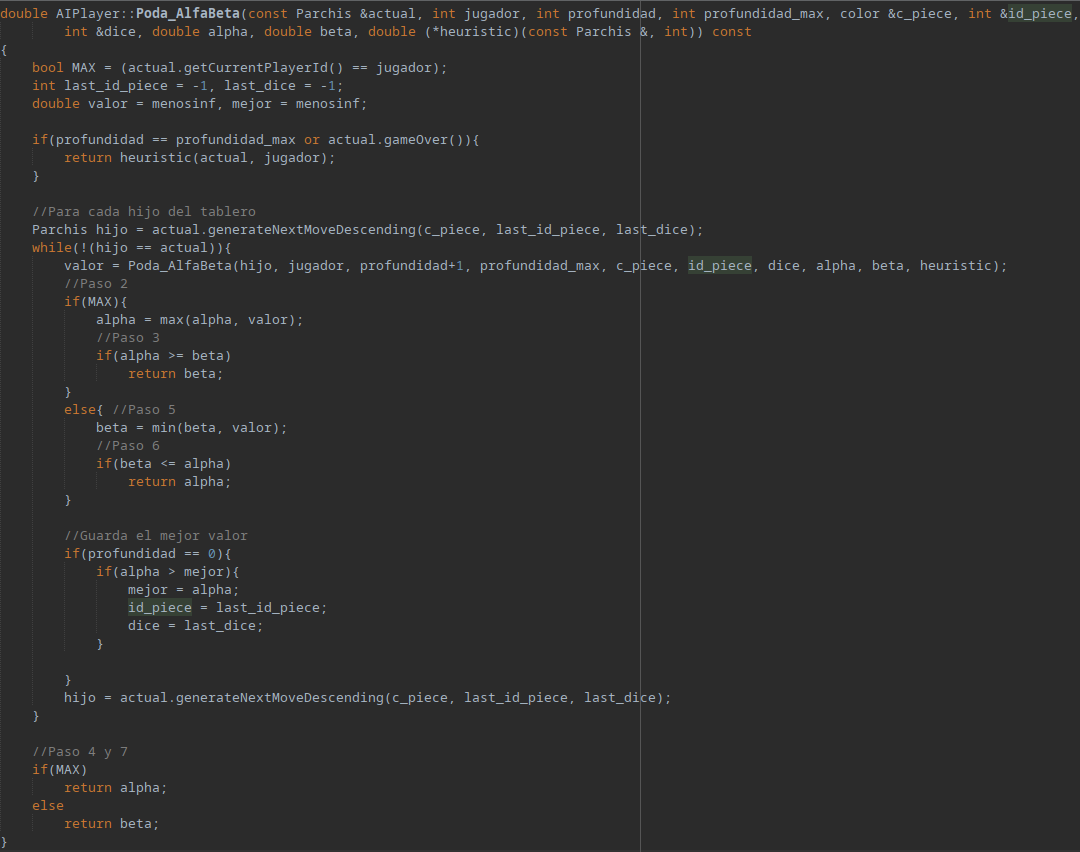
\includegraphics[scale = 0.6]{podaAlfaBeta.png}\\[1.0 cm]\end{centering}

\subsection{Heurísticas}
La heurística es la parte más importante ya que es la que determina el comportamiento del agente que vamos a crear. En mi caso, se dispone de 3 heurísticas muy similares en código pero de comportamientos radicalmente distintos. Las llamaremos ganaJ1, ganaJ2 y valoracionDefinitiva.

\subsubsection{Comportamiento general}
A pesar de ser 3 heurísticas muy distintas, su código es extrañamente similar:
\begin{enumerate}
 \item Si gana el jugador, se devuelve un valor $+\infty$. Si gana el oponente, se devuelve un valor $-\infty$. En otro caso, se establecen las puntuaciones según estados del tablero.

 \item Se recorren todas las fichas del jugador y del oponente con dos bucles for respectivamente: \\ for (i to color.size) for( j to num\_pieces)\{ \emph{puntuaciones} \}

 \item Se valora positivamente la posición de las fichas en el tablero, cuando más alto mejor. Aquí difieren las heurísticas ya que la J1 valora positivamente cualquier posicion del tablero pero las otras 2 solo puntuan si se encuentra en la cola de meta.

 \item Si está en una casilla segura, se valora positivamente. +1 para las J1 y J2, +10 para la definitiva.

 \item Si tiene casillas en casa implica que han sido comidas por lo que se valora muy negativamente. Se resta -100 para cada ficha en home dando como resultado que intenta evitar ser comido y saca fichas cuando puede.

 \item Cualquier casilla que llegue a la meta se puntua de forma muy positiva. Se suma +100 por cada ficha en meta. Al tener la misma puntuación que comer, sigue prefiriendo comer antes que meterla ya que se puntua la posición del tablero positivamente.

 \item La puntuación del oponente es exactamente igual en las 3: Se le valora positivamente al oponente según la posición de sus fichas en el tablero. Además se le penaliza al oponente que sus fichas estén en casa dando como resultado que nuestro agente esté más ansioso por comerselo y bloquear sus casillas de casa (efectivamente, si 2 fichas ocupan la casilla de casa el jugador no puede sacar ficha).


\end{enumerate}


\subsubsection{Heuristicas: ganaJ1}
Esta es la primera heurística y también la que gana de forma aplastante todos los ninjas como jugador 1. Es pésima como jugador 2, no le gana ni al ninja 1.

Su funcionamiento radica en maximizar el desplazamiento en el tablero, cuantas más fichas y mas cerca de la meta haya mejor. Esto le ayuda a alcanzar la meta rapidamente pero deja fichas rezagadas muy golosas para el oponente. Al ser jugador 1 no supone ningun problema ya que se escapa antes de ser comido, no ocurre lo mismo como jugador 2.

\subsubsection{Heuristicas: ganaJ2}
En esta heurística sin embargo les gana de forma aplastante a todos los ninjas como jugador 2. Como jugador 1 dispone de un comportamiento extraño, no vence ni al ninja 1 o 2 pero gana satisfactoriamente contra el ninja 3.

Su funcionamiento radica en valorar muy positivamente la cola de meta pero no el resto del tablero. Esto evita que las fichas queden rezagadas intentando maximizar el tablero, funcionando muy bien como segundo jugador pero no tiende a avanzar por lo que como jugador 1 no es muy buena.

\subsubsection{Heuristicas: valoracionDefinitiva}
Como bien indica su nombre es la que vence de forma satisfactoria a todos los agentes propuestos. Es una heuristica ganaJ2 vitaminada. No vence a los agentes tan sobradamente como las otras 2 por separado.

Es la más distinta de las 3 ya que se añade una funcionalidad extra: detecta enemigos cercanos a cada ficha. Es decir, calcula cuantas fichas enemigas tiene delante y detrás. Puntúa positivamente tener fichas enemigas delante en un rango de 7 casillas, +9. Puntúa negativamente tener fichas enemigas detrás en un rango de 7 casillas, -9. Esta funcionalidad es muy efectiva contra los ninjas 1 y 2 aunque no tanto con el ninja 3 (penaliza tardando más en ganarle).

\section{Conclusiones}
Podemos sacar en claro varias cosas:
\begin{itemize}
 \item En cuanto a comportamiento, a pesar de que las heurísticas son extremadamente simples los agentes desarrollan jugadas complejas. Entre ellas:
 \begin{itemize}
  \item A veces un color obtiene el rol de ``support'' en el que simplemente se dedica a bloquear a las fichas enemigas y ser cebo para el otro color. Mientras que el otro color obtiene el rol de ``ganador'', comiendose toda ficha que ve y llegando rapidamente a la meta.

  \item Suele tender emboscadas en la cual un color bloquea con barrera y otro come fichas.

  \item En determinadas ocasiones las fichas se quedan en las casas de los colores del oponente, impidiendole sacar fichas.

  \item También tiene en cuenta los dados del oponente, colocandose en ``puntos ciegos'' donde el oponente no dispone del número necesario para comer. Destaca el 6, ya que si todas tus fichas están fuera te mueves 7 casillas por lo que toda ficha a distancia 6 necesita de un 5 y un 1.

  \item Es común ver como se come fichas propias con tal de comerse la de otro jugador y llegar antes a la meta. También se come sus propias fichas para entrar directo a la meta o a la cola de meta.

 \end{itemize}

 \item En cuanto al tipo de heuristicas: tanto ganaJ1 como ganaJ2 son heurísticas claramente ofensivas ya que aunque hagan barreras de vez en cuando, intentan moverse rápidamente por el tablero. Sin embargo la heurística definitiva es más equilibrada: tiende a quedarse en zonas seguras e ir avanzando progresivamente pero no desperdicia ninguna oportunidad de comer si le conviene.

 \item Respecto al resto de compañeros, aprovechando la posibilidad de competir entre nosotros he podido comparar mis heurísticas con el resto. En general, se ha optado por heurísticas muy defensivas usando anywall e isWall. Al parecer, este tipo de heurísticas son más efectivas que las ofensivas pues generalmente vencen mi agente (reñidas, eso sí).

 \item El minimax también es capaz de ganar a los 3 agentes como j1 y j2 con la heuristica definitiva aunque con mayor dificultad que el alfa-beta.

\end{itemize}


\vspace{5cm}
 \bibliographystyle{plain}
 \bibliography{biblist}


\end{document}
